\subsubsection{Macro-caso d'uso - Gestione Profilo}
\paragraph{Diagramma UML}

\begin{figure}[H]
    \centering
    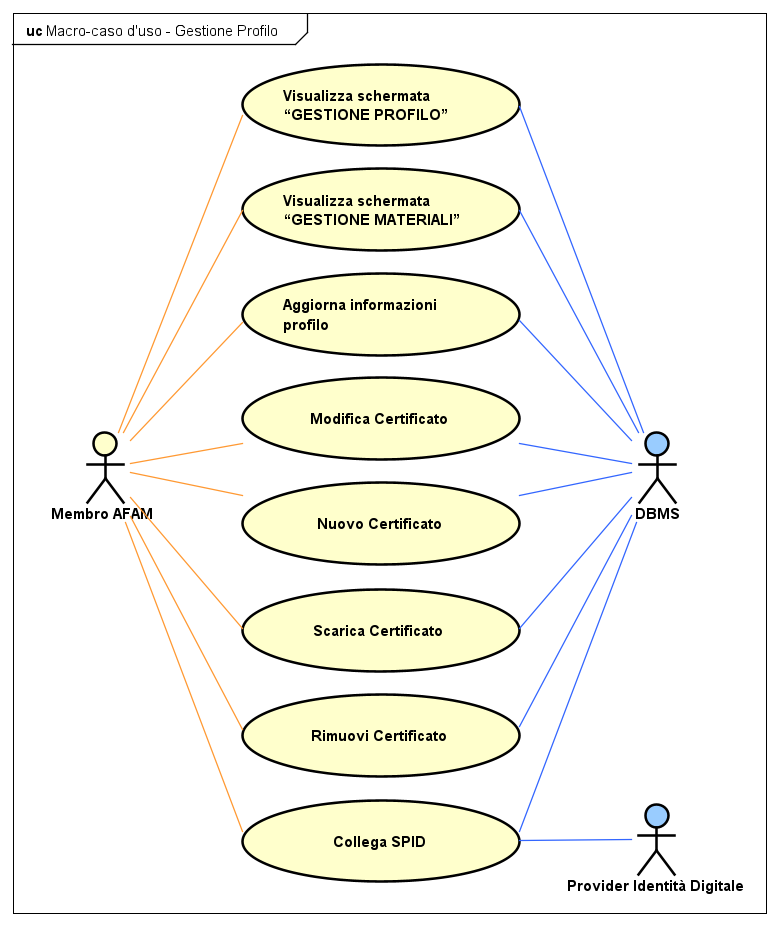
\includegraphics[width=0.95\textwidth, height=0.95\textheight, keepaspectratio]{Immagini/Use-case diagrams/Macro-caso d'uso - Gestione Profilo.png}
\end{figure}

\clearpage

\paragraph{Visualizza schermata ``GESTIONE PROFILO''}
\par{\noindent Questo caso d'uso consente ad un Membro AFAM di accedere alla schermata ``GESTIONE PROFILO'' per gestire i dati personali, associare lo SPID al profilo, gestire gli attestati e chiudere l'account.}

\begin{tabularx}{\textwidth}{|C|X|}
\hline
\rigaTabella{Caso d'uso}{Visualizza schermata ``GESTIONE PROFILO''}
\rigaTabella{ID}{VIS\_SCH\_GES\_PRO}
\rigaTabella{Attori}{Membro AFAM, DBMS}
\rigaTabella{Precondizione}{Il sistema ha mostrato la schermata ``HOME''}
\rigaTabella{Flusso degli eventi}{\begin{enumerate}
    \item Il Membro clicca il pulsante ``PROFILO''
    \item Il sistema interroga il DBMS per ottenere le informazioni del Membro
    \item Il sistema mostra a video la schermata ``GESTIONE PROFILO''
\end{enumerate}
}
\rigaTabella{Postcondizione}{Il sistema ha mostrato a video la schermata ``GESTIONE PROFILO''}
\hline
\end{tabularx}

\paragraph{Visualizza schermata ``GESTIONE CERTIFICATI''}
\par{\noindent Questo caso d'uso consente ad un Membro AFAM di accedere alla schermata ``GESTIONE CERTIFICATI'' per gestire gli attestati creandone di nuovi, scaricarli e cancellarli.}

\begin{tabularx}{\textwidth}{|C|X|}
\hline
\rigaTabella{Caso d'uso}{Visualizza schermata ``GESTIONE CERTIFICATI''}
\rigaTabella{ID}{VIS\_SCH\_GES\_CERT}
\rigaTabella{Attori}{Membro AFAM, DBMS}
\rigaTabella{Precondizione}{Il sistema ha mostrato la schermata ``HOME''}
\rigaTabella{Flusso degli eventi}{\begin{enumerate}
    \item Il Membro clicca il pulsante ``CERTIFICATI''
    \item Il sistema interroga il DBMS per ottenere i certificati del Membro
    \item Il sistema mostra a video la schermata ``GESTIONE CERTIFICATI''
\end{enumerate}
}
\rigaTabella{Postcondizione}{Il sistema ha mostrato a video la schermata ``GESTIONE CERTIFICATI''}
\hline
\end{tabularx}

\clearpage

\paragraph{Aggiorna Informazioni Profilo}
\par{\noindent Questo caso d'uso permette al Membro AFAM di modificare e aggiornare i dati anagrafici, i contatti professionali, i link social e le impostazioni di privacy del proprio account.}

\begin{tabularx}{\textwidth}{|C|X|}
\hline
\rigaTabella{Caso d'uso}{Aggiorna Informazioni Profilo}
\rigaTabella{ID}{UPD\_INF\_PRO}
\rigaTabella{Attori}{Membro AFAM, DBMS}
\rigaTabella{Precondizione}{Il sistema ha mostrato la schermata ``GESTIONE PROFILO''}
\rigaTabella{Flusso degli eventi}{\begin{enumerate}
    \item Il Membro immette le nuove informazioni
    \item Il Membro clicca il pulsante ``SALVA'' \label{Salva informazioni}
    \item Il sistema controlla se la data di nascita \`e superiore a quella corrente
    \item \textbf{FINCH\'E} la data di nascita \`e superiore a quella corrente:
    \begin{enumerate}
        \item Il sistema mostra a video l'errore: ``Errore: Data errata''
        \item Il Membro ricompila i campi
        \item Il Membro clicca il tasto ``SALVA''
        \item Il sistema controlla se la data di nascita \`e superiore a quella corrente
    \end{enumerate}
    \item Il sistema interroga il DBMS per aggiornare le informazioni
    \item Il sistema mostra il messaggio: ``Informazioni aggiornate con successo''
    \item Il sistema mostra la schermata ``GESTIONE PROFILO'' aggiornata
\end{enumerate}
}
\rigaTabella{Sequenza alternative}{
    \begin{enumerate}[start=2]
        \item Il Membro clicca sull'immagine profilo
        \item Il sistema mostra l'esplora file del dispositivo su cui si trova il Membro
        \item Il Membro seleziona l'immagine da caricare
        \item Il sistema interroga il DBMS per aggiornare l'immagine del profilo
    \end{enumerate}
    Il flusso riprende dal punto \ref{Salva informazioni}
}
\rigaTabella{Postcondizione}{Il sistema ha mostrato la schermata ``GESTIONE PROFILO'' aggiornata}
\rigaTabella{Requisiti Speciali}{I dati informativi che compongono il profilo sono:
\begin{itemize}
    \item Nome, Cognome, Data di nascita, Luogo di nascita
    \item Foto profilo, Indirizzo, Professione, Numero di telefono
    \item Indirizzo email, Indirizzo email per contatti
    \item Profilo Instagram, Profilo LinkedIn, Profilo Facebook
    \item Impostazione Account (Pubblico o Privato)
    \item Impostazione ricezione condivisioni
\end{itemize}
Il pulsante ``SALVA'' è disabilitato se non sono stati modificate le informazioni o se dei campi sono rimasti vuoti}
\hline
\end{tabularx}

\clearpage

\paragraph{Nuovo certificato}
\par{\noindent Questo caso d'uso permette ad un Membro AFAM di inserire un nuovo certificato tramite la schermata ``GESTIONE CERTIFICATI'', verificando il rispetto dei vincoli di formato e dimensione previsti dalla piattaforma.}

\begin{tabularx}{\textwidth}{|C|X|}
\hline
\rigaTabella{Caso d'uso}{Nuovo certificato}
\rigaTabella{ID}{NUO\_CER}
\rigaTabella{Attori}{Membro AFAM, DBMS}
\rigaTabella{Precondizione}{Il sistema ha mostrato la schermata ``GESTIONE CERTIFICATI''}
\rigaTabella{Flusso degli eventi}{\begin{enumerate}
    \item Il Membro clicca il pulsante ``NUOVO''
    \item Il sistema mostra la modale ``NUOVO CERTIFICATO''
    \item Il Membro inserisce titolo e visibilit\`a
    \item Il Membro clicca sul riquadro per caricare l'attestato
    \item Il sistema mostra l'esplora file del dispositivo su cui si trova il Membro
    \item Il Membro seleziona il Materiale da caricare
    \item Il Membro clicca il tasto ``SALVA'' \label{salva attestato}
    \item Il sistema controlla la correttezza dell'attestato
    \item \textbf{FINCH\`E} l'attestato non rispetta le dimensioni specifiche:
    \begin{enumerate}
        \item Il sistema mostra a video l'errore: ``Errore: File troppo grande''
        \item Il Membro ricarica l'attestato
        \item Il Membro clicca il tasto ``SALVA''
        \item Il sistema controlla la correttezza dell'attestato
    \end{enumerate}
    \item Il sistema interroga il DBMS per salvare il Certificato
    \item Il sistema interroga il DBMS per ottenere la lista dei Certificati aggiornata
    \item Il sistema mostra la schermata ``GESTIONE CERTIFICATI'' aggiornata
\end{enumerate}
}
\rigaTabella{Sequenze alternative}{
\begin{enumerate}[start=4]
    \item Alternativamente il Membro trascina il Materiale da caricare all'interno del riquadro. Il flusso riprende dal punto \ref{salva attestato}
\end{enumerate}
}
\rigaTabella{Postcondizione}{Il sistema ha mostrato la schermata ``GESTIONE CERTIFICATI'' aggiornata.}
\rigaTabella{Requisiti Speciali}{Finch\`e il titolo \`e vuoto il pulsante salva \`e disabilitato. \newline 
Le dimensioni massime per ogni singolo attestato sono 50 megabyte. \newline
I formati validi per gli attestati sono: [PDF, PNG, JPG]. \newline
Le informazioni complementari sono composte da: Titolo, Pubblico o privato.}
\hline
\end{tabularx}

\clearpage

\paragraph{Scarica Certificato}
\par{\noindent Il seguente caso d'uso permette al Membro AFAM di scaricare i certificati precedentemente caricati.}

\begin{tabularx}{\textwidth}{|C|X|}
\hline
\rigaTabella{Caso d'uso}{Scarica Certificato}
\rigaTabella{ID}{SCA\_CERT}
\rigaTabella{Attori}{Membro AFAM, DBMS}
\rigaTabella{Precondizione}{Il sistema ha mostrato la schermata ``GESTIONE CERTIFICATI''}
\rigaTabella{Flusso degli eventi}{\begin{enumerate}
    \item Il Membro seleziona uno o pi\`u Certificati dalla lista
    \item Il Membro clicca il pulsante ``SCARICA''
    \item \textbf{PER OGNI} Certificato selezionato:
    \begin{enumerate}
        \item Il sistema interroga il DBMS per ottenere il Certificato da scaricare
        \item Il sistema scarica il Certificato
    \end{enumerate}
\end{enumerate}
}
\rigaTabella{Postcondizione}{}
\end{tabularx}

\clearpage

\paragraph{Rimuovi Certificato}
\par{\noindent Il seguente caso d'uso permette al Membro AFAM di rimuovere i certificati che aveva precedentemente caricato.}

\begin{tabularx}{\textwidth}{|C|X|}
\hline
\rigaTabella{Caso d'uso}{Rimuovi Certificato}
\rigaTabella{ID}{RIM\_CERT}
\rigaTabella{Attori}{Membro AFAM, DBMS}
\rigaTabella{Precondizione}{Il sistema ha mostrato la schermata ``GESTIONE CERTIFICATI''}
\rigaTabella{Flusso degli eventi}{\begin{enumerate}
    \item Il Membro seleziona uno o pi\`u Certificati dalla lista
    \item Il Membro clicca il pulsante per cancellare
    \item \textbf{PER OGNI} Certificato selezionato:
    \begin{enumerate}
        \item Il sistema interroga il DBMS per cancellare il Certificato selezionato
    \end{enumerate}
    \item Il sistema interroga il DBMS per ottenere la lista dei Certificati aggiornata
    \item Il sistema mostra a video la schermata ``GESTIONE CERTIFICATI'' aggiornata
\end{enumerate}
}
\rigaTabella{Postcondizione}{Il sistema ha mostrato la schermata ``GESTIONE CERTIFICATI'' aggiornata}
\end{tabularx}

\clearpage

\paragraph{Modifica Certificato}
\par{\noindent Questo caso d'uso permette al Membro AFAM di modificare le informazioni relative a un attestato precedentemente caricato, aggiornando il titolo o variandone lo stato di visibilit\`a all'interno della schermata di gestione.}

\begin{tabularx}{\textwidth}{|C|X|}
\hline
\rigaTabella{Caso d'uso}{Modifica Certificato}
\rigaTabella{ID}{UPD\_CERT}
\rigaTabella{Attori}{Membro AFAM, DBMS}
\rigaTabella{Precondizione}{Il sistema ha mostrato la schermata ``GESTIONE CERTIFICATI''}
\rigaTabella{Flusso degli eventi}{\begin{enumerate}
    \item Il Membro seleziona il Certificato di cui vuole modificare i dettagli
    \item Il Membro clicca il pulsante ``MODIFICA''
    \item Il sistema mostra la modale ``MODIFICA CERTIFICATO''
    \item Il Membro inserisce il nuovo titolo e opzionalmente modifica la visibilit\`a del Certificato
    \item Il Membro clicca il tasto ``SALVA''
    \item Il sistema interroga il DBMS per aggiornare i dettagli del Certificato
    \item Il sistema interroga il DBMS per ottenere la lista dei Certificati aggiornata
    \item Il sistema mostra la schermata ``GESTIONE CERTIFICATI'' aggiornata
\end{enumerate}
}
\rigaTabella{Postcondizione}{Il sistema ha mostrato la schermata ``GESTIONE CERTIFICATI'' aggiornata}
\rigaTabella{Note}{Il pulsante ``SALVA'' \`e disabilitato se il campo titolo e la visibilit\`a non sono stati modificati o se il campo titolo \`e vuoto.}
\hline
\end{tabularx}

\clearpage

\paragraph{Collega SPID}
\par{\noindent Il presente caso d'uso permette al Membro AFAM di associare il proprio SPID per verificare il propio profilo.}

\begin{tabularx}{\textwidth}{|C|X|}
\hline
\rigaTabella{Caso d'uso}{Collega SPID}
\rigaTabella{ID}{COL\_SPID}
\rigaTabella{Attori}{Membro AFAM, Provider Identit\`a digitale, DBMS}
\rigaTabella{Precondizione}{Il sistema ha mostrato la schermata ``GESTIONE PROFILO''}
\rigaTabella{Flusso degli eventi}{\begin{enumerate}
    \item Il Membro clicca sul pulsante ``COLLEGA SPID''
    \item Il sistema mostra un menu con i provider di identit\`a digitale
    \item Il Membro seleziona il proprio provider
    \item Il sistema mostra a video la schermata di autenticazione del provider
    \item Il Membro si autentica
    \item \textbf{SE} l'autenticazione presso il provider non va a buon fine:
    \begin{enumerate}
        \item Il sistema mostra a video la schermata ``GESTIONE PROFILO''
        \item Il sistema mostra a video l'errore: ``Errore: Impossibile contattare il provider''
    \end{enumerate}
    \item \textbf{ALTRIMENTI}:
    \begin{enumerate}
        \item Il sistema ottiene dal provider i dati del Membro
        \item Il sistema interroga il DBMS per associare lo spid al Membro
        \item Il sistema mostra a video la schermata ``GESTIONE PROFILO''
    \end{enumerate}
\end{enumerate}
}
\rigaTabella{Postcondizione}{Il sistema ha mostrato la schermata ``GESTIONE PROFILO''}
\rigaTabella{Note}{Quando il Membro collega lo SPID le informazioni anagrafiche vengono sostituite da quelle che restituisce il provider, verificando inoltre l'account del Membro. Il pulsante ``COLLEGA SPID'' mostrer\`a quindi la scritta ``SPID COLLEGATO''.}
\hline
\end{tabularx}

\clearpage